\documentclass{standalone}
\usepackage{tikz}
\usepackage{tikz-feynman} % Paquete para diagramas de Feynman
\begin{document}

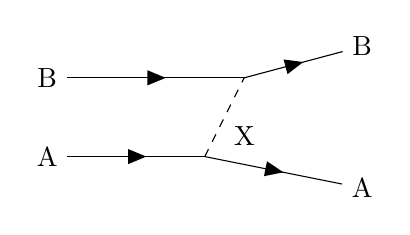
\begin{tikzpicture}
    \begin{feynman}
        % Nodos de partículas
        \vertex (i1) at (-1,1) {A};
        \vertex (v1) at (1,1);
        \vertex (f1) at (3,0.6) {A};
        \vertex (v2) at (1.5,2);
        \vertex (i2) at (-1,2) {B};
        \vertex (f2) at (3,2.4) {B};
        
        % Diagramas de líneas
        \diagram* {
            (i1) -- [fermion] (v1), % Línea A
            (v1) -- [fermion] (f1), % Línea del electrón desviado
            (i2) -- [fermion] (v2), % Línea B
            (v2) -- [fermion] (f2), % Línea del electrón desviado
            (v1) --[dashed, edge label' = X] (v2); % Línea punteada con etiqueta X
        };
    \end{feynman}
\end{tikzpicture}

\end{document}
